\documentclass{article}
\usepackage[T1]{fontenc}
\usepackage{lmodern}
\usepackage{graphicx}
\usepackage{amsmath,amssymb}
\usepackage[a4paper,margin=2cm]{geometry}
\usepackage[absolute,overlay]{textpos}
\setlength{\TPHorizModule}{1mm}
\setlength{\TPVertModule}{1mm}
\usepackage[indonesian]{babel}
\usepackage{hyperref}
\setlength{\emergencystretch}{2em}
% unit: Halaman 111

\begin{document}

% === Halaman 111 (python/native) ===

111

• Enigma  menggunakan sistem rotor (roda 

berputar) untuk membentuk huruf 

cipherteks yang berubah-ubah.

• Setiap rotor melakukan substitusi abjad-

tunggal (monoalphabetic cipher).

• Hasil substitusi oleh suatu rotor menjadi 

huruf input untuk operasi substitusi rotor 

selanjutnya.

• Hasil substitusi oleh rotor terakhir menjadi 

huruf cipherteks.

• Setiap kali sebuah huruf dienkripsi oleh 

sebuah rotor, rotor  berputar satu huruf 

untuk membentuk huruf cipherteks baru 

bagi huruf plainteks berikutnya. 

• Setelah berputar 26 huruf rotor kembali 

pada posisi semula. Jadi, diperoleh cipher 

abjad-majemuk dengan periode 26.

% deskripsi: gambar native xref 399
\noindent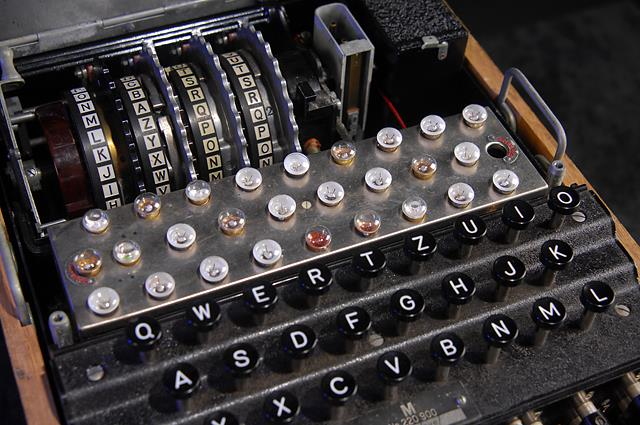
\includegraphics[width=0.85\textwidth]{../../images/python/page_111_img_01.jpeg}

\end{document}
